\label{chapter:metodo}
\par
Neste capítulo descreve o método proposto utilizado no desenvolvimento deste projeto. Inicialmente será apresentado o modelo geral e posteriormente as duas abordagens utilizadas com base neste método, além dos pontos principais de cada uma delas. Ambos os métodos são baseados em transformações de códigos para análise de circuitos lógicos descritos em VHDL utilizando 
\textit{Bounded Model Checking}, neste caso o \textit{model checker} ESBMC.

%======================
%Visão geral do método
%======================
\section{Visão geral}

\par
O método proposto consiste na análise de códigos VHDL através da inserção de assertivas ao código, de modo a validar ou mesmo gerar a ocorrência de erros que possam ocorrer durante a execução. Aliado a inserção de assertivas, também é utilizado a técnica de transformação de código, convertendo o mesmo de VHDL para linguagem C. 

\begin{figure}[H]
	\begin{center}
    \caption{\label{fig:metodo} Fluxograma do método proposto.}
	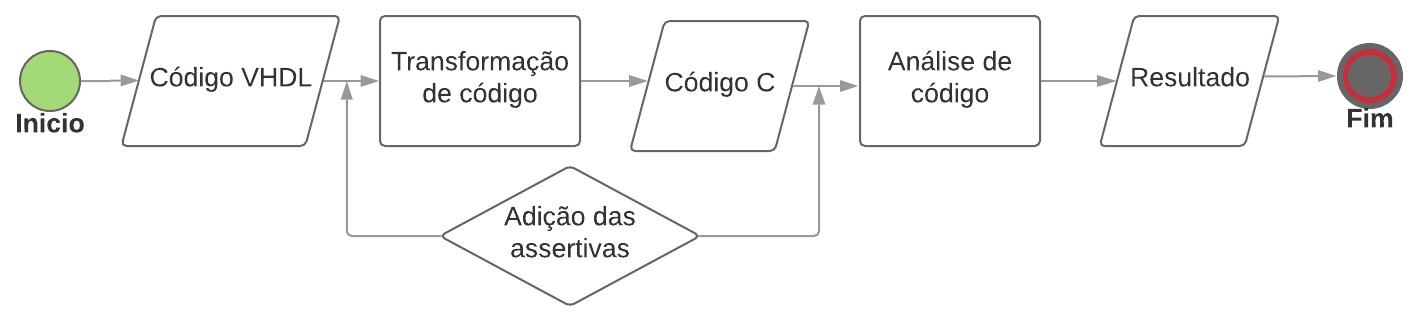
\includegraphics[scale=0.32]{Figuras/Fluxo_metodo.png}
	\end{center}
    \legend{Fonte:Própria}
\end{figure}

\par
Partindo do citado anteriormente e conforme mostrado na \autoref{fig:metodo}, o método se inicia com o código em VHDL a ser analisado. Nenhuma analise é realizada diretamente sobre o código VHDL, sendo apenas sobre o código já convertido para linguagem C, devido a existência de vários analisadores de código que são utilizados para identificação de erros nesta linguagem, por exemplo, a ferramenta ESBMC. 

\par
As assertivas podem ser inseridas antes ou depois da transformação de código. Independente do caso adotado, a mesma devem seguir o padrão aceito pela ferramenta de analise utilizada, caso contrário, a mesma não apresentará a eficácia necessária. A escolha do momento de inserção das assertivas depende principalmente do modo como a tradução ta sendo realizada e as capacidades da ferramenta de tradução em converter estas assertivas.

\par
Sendo as assertivas inseridas antes da transformação, mesma deve ser traduzida para linguagem C, seja pela ferramenta, na forma de comentário ou por meio de alguma instrumentação que venha a ser realizada no código. Esta instrumentação não deve alterar a lógica do código, pois desta forma a mesma alteraria o código que pretende ser analisado. Caso seja feita após a tradução, a mesma já pode ser inserida ao código diretamente em linguagem C.

\par
O analisador deve ser capaz de interpretar as assertivas adicionadas ao código, deste modo, um padrão deve ser implementado de acordo com as particularidades da ferramenta, neste caso, de acordo com as funções da ferramenta de análise. Deste modo, evita que erros possam ocorrer durante a análise do código.
%++++++++++++++++++++++++++++++++++++++++++++++++++++++++++
%==========================================================
%APRESENTAÇÃO DAS ABORDAGENS
%==========================================================
%++++++++++++++++++++++++++++++++++++++++++++++++++++++++++
\section{Abordagens desenvolvidas}
%\par
%Inicialmente será apresentado o método de transformação direta e todas as suas etapas e posteriormente será a presentado o método de múltiplas transformações. Com o intuito de auxiliar nas explicações apresentadas nas próximas seções, o código na \autoref{fig:code_exemplo} será utilizado nas explanações, bem como será apresentado todas as alterações do mesmo, conforme cada etapa do método. 

%\todo[inline]{Adicionar explicação que séra apresentado apenas os modelos de tradução e que a analise de código será a mesma utilizada nos dois métodos}

\par
Inicialmente será apresentado dois métodos de tradução que foram desenvolvidos durante a elaboração do trabalho. Ambos os métodos foram baseados na estrutura geral do método, utilizando o sistema de assertivas, ferramentas de transformação. Para o total funcionamento das abordagens, são realizadas instrumentações para adaptação do códigos com as ferramentas e também na execucão das mesmas. 

\par
O primeiro método chamado de transformação direta apresenta uma unica ferramenta que realizada a conversão de VHDL para C. O circuito lógico descrito em VHDL, onde as assertivas serão inseridas pelo próprio usuário do método. O código VHDL é traduzido para linguagem C e recebe uma instrumentação de código para a posterior validação do mesmo. O Código em C automaticamente gerado será processado e analisado, e de acordo com as assertivas inseridas, apresentará falha, caso alguma delas seja violada. 

\par
O segundo método chamado de multiplas trasnformações apresenta duas ferramentas de transformação, sendo a primeira de VHDL para Verilog e seguido de uma ferramenta de Verilog para C. Inicialmente o código em VHDL é passado para ferramenta juntamente com outro arquivo contendo as variáveis de entrada, saída, pré-condições e pós-condições. Seguidamente é passado para duas ferramenta de tradução e também duas etapas de instrumentação. Após as traduções, as pré-condições e pós-condições, conforme o arquivo, são adicionadas ao códigos C e o mesmo é analisado. Caso alguma condição seja violada, o contra exemplo é apresentado ao usuário.

\par
A parte referênte a analise do código será apresentada em uma única sessão, visto que ambas as abordagens apresenta a mesma ferramenta para analise e estruturas. Será demonstrado de que forma a ferramenta foi utilizada para verificação da corretude do código, através das assertivas. 

\par
O código é um conceito básico de ula, formado apenas pelas portas AND e OR, além de um inversor o qual inverte o sinal de entrada, caso seja necessário. A saída deste inversor é ligada as portas AND e OR, e a saída desta porta é ligada a um multiplexador de duas entradas. Ao final, a saída do multiplexador será um dos sinais de entrada, ou seja, ou o sinal enviado pela porta AND ou pela porta OR e este sinal de saída será determinado de acordo com o sinal de escolha enviado ao multiplexador.

\begin{figure}[H]
\caption{\label{fig:code_exemplo} Exemplo de código VHDL de ULA com portas AND e OR.}
	\begin{center}
    \begin{minipage}{0.7\textwidth}
    \begin{lstlisting}       
library ieee;
use ieee.std_logic_1164.all;

ENTITY Ula_tcc IS
PORT(A,B,Binvertido,Op1:IN std_logic;
	  Resultado:OUT std_logic);
END Ula_tcc;

ARCHITECTURE Ula_tcc_behavl OF Ula_tcc IS
SIGNAL and_port: std_logic;
SIGNAL or_port: std_logic;
SIGNAL mux2x1: std_logic;
BEGIN
	PROCESS(A,B,Binvertido,Op1)
	BEGIN
		IF(Binvertido = '0') THEN
			mux2x1 <= B;
		ELSE
			mux2x1 <= NOT B;
		END IF;
		and_port <= A AND mux2x1;
		or_port <= A OR mux2x1;
		IF(Op1 = '0') THEN
			Resultado <= and_port;
		ELSIF(Op1 = '1') THEN
			Resultado <= or_port;
		END IF;
	END PROCESS;
END Ula_tcc_behavl;
    \end{lstlisting}
    \end{minipage}
	\end{center}
    \legend{Fonte: Própria.}
\end{figure}

\subsection{Método de transformação direta}
%==========================================================
%Visão geral do método de transformação direta
%==========================================================
%\subsection{Visão geral do método de transformação direta}
%\par
%O método proposto consiste inicialmente em receber como entrada um circuito lógico descrito em VHDL, onde uma dada propriedade representada em uma assertiva será analisada, as assertivas serão inseridas de automaticamente pelo método ou pelo próprio usuário do método. O código VHDL analisado posteriomente é traduzido para linguagem C e recebe uma instrumentação de código (com funções especificas suportadas pelo método) para a posterior validação do mesmo. O Código em C automaticamente gerado, já instrumentado, será processado e analisado pelo ESBMC de acordo com as assertivas inseridas e ao final é apresentado o resultado. Caso alguma das assertivas seja violada, um contra-exemplo é apresentado ao usuário.

\subsubsection{Preprocessamento do VHDL e inserção de assertivas}

\par
A fase inicial do método consiste na adição das assertivas ao código VHDL. Vale ressaltar que mesmo a linguagem VHDL tendo um modelo de assertivas, tornou-se necessário a criação de um modelo próprio, baseado em comentários, para que as funções do model checker adotado fossem suportadas, como a geração de valores não determinísticos.\todo{Adicionar significado do termo} 

\par
As assertivas são adicionadas entre as tags \texttt{@c2vhdl:ASSERT} e \texttt{@c2vhdl:END} e todo trecho de código entre estas tags deve estar comentado, desta forma não apresentará erro na tradução do código em linguagem C, bem como na sintetização do código VHDL. Nas assertivas são incluídas as funções necessárias para a análise utilizando a ferramenta ESBMC. A assertiva apresenta três informações principais, sendo elas: condição, mensagem e gravidade. 

\begin{figure}[H]
\caption{\label{fig:assertiva} Exemplo de assertiva para verificação de porta \texttt{AND}.}
	\begin{center}
    \begin{minipage}{0.99\textwidth}
    \begin{lstlisting}       
--@c2vhdl:ASSERT
--assert (Resultado = '1')
--report "O resutado foi diferente a 0"
--severity ERROR;
--@c2vhdl:END
    \end{lstlisting}
    \end{minipage}
	\end{center}
    \legend{Fonte: Própria.}
\end{figure}

\par
A condição, \textbf{linha $2$} da \autoref{fig:assertiva}, representa a assertiva propriamente dita e que será analisado pela aplicação. A condição será precedida de \texttt{$--$assert} e seguido ou não da palavra \texttt{not}, com isso a assertiva pode assumir valor negativo, conforme necessidade do usuário. Na \autoref{fig:assertiva} a assertiva busca verificar se a variável \texttt{Resultado} terá valor igual a $1$, com isso ao comparar o valor buscado pela assertiva e o gerado no final do código, caso ambos sejam iguais, ocorre falha na verificação. 

\par
A mensagem, \textbf{linha $3$} da \autoref{fig:assertiva}, é definida pelo usuário e será exibida caso a assertiva apresente falha, assim a mensagem pode ser utilizada como um meio de depuração das propriedades validadas. A severidade, \textbf{linha $2$} da \autoref{fig:assertiva}, pode ser definida como \texttt{error}, que representa um erro fatal e parada da verificação. A severidade do tipo \texttt{warning} que representa um erro não fatal, contabiliza as falhas das assertivas, porém não causa a parada da verificação.

\par
Juntamente com as assertivas outra função que pode ser utilizada é a função \texttt{\_\_ESBMC\allowbreak{}\_assume()} suportada pelo model checker ESBMC. Esta função utilizada em conjunto com a ferramenta ESBMC permite que durante a verificação uma variável possa ter um valor definido durante o tempo de execução da verificação. A importância desta função é fazer verificações onde se conhece os valores de entrada juntamente com o valor resultante, por exemplo, na verificação de portas lógicas.

\begin{figure}[H]
\caption{\label{fig:assertiva_assume} Exemplo de utilização da função \texttt{\_\_ESBMC\_assume()}.}
	\begin{center}
    \begin{minipage}{0.99\textwidth}
    \begin{lstlisting}       
    --__ESBMC_assume(A = '0');
    --__ESBMC_assume(B = '1');
    --__ESBMC_assume(Binvertido = '1');
    --__ESBMC_assume(Op1 = '0');
    \end{lstlisting}
    \end{minipage}
	\end{center}
    \legend{Fonte: Própria.}
\end{figure}

\par
%A assertivas que serão verificadas são automáticas traduzidas a partir das entradas do código VHDL. Seja no modelo manual (assertivas escritas pelo usuário) ou automático (inferidas pelo método proposto por meio de análise estática), as entradas são mapeadas para serem utilizados na etapa de instrumentação. Desta forma, tais entradas podem ser utilizadas para gerar essas assertivas e então serem adicionadas diretamente ao código em linguagem C durante a fase de instrumentação.

\par
Na \autoref{fig:code_assertivas} apresenta o código exemplo da \autoref{fig:code_exemplo}. Nele já encontram inserido os \textit{\_\_ESBMC\_assume()} anterior ao código para inicializar as variaveis necessárias e as assertivas após todo o código, de modo que a assertiva permaneça ao final do código.

\begin{figure}[H]
\caption{\label{fig:code_assertivas} Exemplo da \autoref{fig:code_exemplo} com assertiva}
	\begin{center}
    \begin{minipage}{0.7\textwidth}
    \begin{lstlisting}       
library ieee;
use ieee.std_logic_1164.all;

ENTITY Ula_tcc IS
PORT(A,B,Binvertido,Op1:IN std_logic;
	  Resultado:OUT std_logic);
END Ula_tcc;

ARCHITECTURE Ula_tcc_behavl OF Ula_tcc IS
SIGNAL and_port: std_logic;
SIGNAL or_port: std_logic;
SIGNAL mux2x1: std_logic;
BEGIN
	PROCESS(A,B,Binvertido,Op1)
	--__ESBMC_assume(A = '0');
  --__ESBMC_assume(B = '1');
  --__ESBMC_assume(Binvertido = '1');
  --__ESBMC_assume(Op1 = '0');
	BEGIN
		IF(Binvertido = '0') THEN
			mux2x1 <= B;
		ELSE
			mux2x1 <= NOT B;
		END IF;
		and_port <= A AND mux2x1;
		or_port <= A OR mux2x1;
		IF(Op1 = '0') THEN
			Resultado <= and_port;
		ELSIF(Op1 = '1') THEN
			Resultado <= or_port;
		END IF;
	    --@c2vhdl:ASSERT
    --assert (Resultado = '1')
    --report "O resutado foi diferente a 0"
    --severity ERROR;
    --@c2vhdl:END
	END PROCESS;
END Ula_tcc_behavl;
    \end{lstlisting}
    \end{minipage}
	\end{center}
    \legend{Fonte: Própria.}
\end{figure}
%=========================================================
%Tradução de código VHDL para a linguagem C
%=========================================================
\subsubsection{Tradução de código VHDL para a linguagem C}
\par
Nesta etapa a tradução do código VHDL para linguagem C é executada. A partir deste ponto, a ferramenta é executada de maneira propriamente dita, tendo todo o processo automatizado até a apresentação do resultado. Para esta etapa do método foi selecionado a ferramenta V2C\cite{albertoV2C} que realiza a tradução de VHDL para Linguagem C.

\par
A ferramenta V2C apresenta diversas vantagens em relação a equivalência de tradução de linguagens, contudo V2C apresenta certas limitações na tradução do código VHDL, em outras palavras, a mesma não reconhece algumas estruturas específicas do VHDL. A ferramenta aceita apenas entradas e saídas do tipo: \texttt{bit}, \texttt{std\_ulogic}, \texttt{qsim\_state}, \texttt{std\_ulogic\_vector} e \texttt{interger}. Na parte de arquitetura, a ferramenta aceita uma gama maior de estruturas, trabalhando com expressões do tipo: \texttt{signal}, \texttt{variable}, \texttt{integers}, \texttt{strings} e caracteres. Em expressões condicionais os operandos são \texttt{AND}, \texttt{OR}, \texttt{NOT} $<=$, $=>$,$=$,$<$,$>$ e $<>$. Aceita também a estrutura de \texttt{process}, além da estrutura \texttt{block}. A estrutura \texttt{process} é limitada apenas a: \texttt{if-else}, \texttt{case} e \texttt{loops}. Como trabalho futuro, neste trabalho tem-se buscado novas abordagens para ampliar o suporte a estruturas não suportadas pelo V2C.

\par
Na tradução é necessário substituir os operadores originais por seus equivalentes em linguagem C. A exceção são os operadores específicos que gerenciam os valores de \texttt{bit}, tais como concatenação ou manipulação de partes vetores, para os quais são necessários construir procedimentos específicos em C.

Na tradução são gerados vários vetores para suporte a tradução dos sinais representados no VHDL, sendo eles \texttt{chg[]}, \texttt{old[]} e \texttt{new[]}. O vetor \texttt{old[]} contém o valor dos sinais do ciclo anterior e operação e a partir deste vetor, o valor a ser usado nos cálculos posteriores é obtido. O vetor \texttt{new[]} representa os novos valores que foram calculados durante a execução do ciclo e este novos são calculados pelos antigos existentes no vetor \texttt{old[]}. E o vetor \texttt{chg[]} contém um or exclusivo entre o valor novo e antigo e em caso de alteração entre os valores é copiado o valor de \texttt{new[]} para \texttt{old[]}.

\par
No código C gerado, os vetores \texttt{in\_data[]} e \texttt{out\_data[]} contêm os sinais de entrada e saída, respectivamente. No caso de circuitos sequenciais, o valor do status é inserido no primeiro (índice 0). A ferramenta lerá os valores \texttt{in\_data[]} e escreverá os resultados do processamento em \texttt{out\_data[]}. Ao final da operação os valores de estado finais salvos no vetor \texttt{new[]} são passados para \texttt{out\_data[]}.

\par
Conforme especificado e seguindo os parâmetros da ferramenta, a mesma realiza a tradução, mantendo inalterado qualquer fragmento de código que esteja comentado, neste caso, as assertivas presentes no código VHDL permanecem inalteradas, sendo utilizadas na próxima etapa do método proposto.

\begin{figure}[H]
\caption{\label{fig:code_trad} Exemplo da \autoref{fig:code_assertivas} traduzido para linguagem C}
	\begin{center}
    \begin{minipage}{0.7\textwidth}
    \begin{lstlisting}       
[...]
   /* Start of Translation */

   /* p0: */
   if (chg[A] || chg[B] || chg[Binvertido] || chg[Op1]) {
      /*__ESBMC_assume(A = '0');
       *__ESBMC_assume(B = '1');
       *__ESBMC_assume(Binvertido = '1'); 
       *__ESBMC_assume(Op1 = '0'); */
            if ((old[Binvertido]==0)) {
         if (chg[B]) {
            new[mux2x1]=old[B];
            }
         }
      else {
         if (chg[B]) {
            new[mux2x1]=~old[B];
            }
         }
      if (chg[A] || chg[mux2x1]) {
         new[and_port]=old[A] & old[mux2x1];
         }
      if (chg[A] || chg[mux2x1]) {
         new[or_port]=old[A] | old[mux2x1];
         }
      if ((old[Op1]==0)) {
         if (chg[and_port]) {
            new[Resultado]=old[and_port];
            }
         }
      else if ((old[Op1]==1)) {
         if (chg[or_port]) {
            new[Resultado]=old[or_port];
            }
         }
      /*@c2vhdl:ASSERT
       *assert (Resultado = '1')
       *report "O resutado foi diferente a 0"
       *severity ERROR;
       *@c2vhdl:END */
      }
   /* End of Translation */
   [...]
    \end{lstlisting}
    \end{minipage}
	\end{center}
    \legend{Fonte: Própria.}
\end{figure}

%========================
%Instrumentação de código
%========================
\subsubsection{Instrumentação de código}

\par
As assertivas após a tradução permanecem comentadas, sendo necessário preparar-las, ou seja traduzi-las, para verificação posterior do código na linguagem em C. Com isso é necessário uma instrumentação do código para prover suporte as assertivas traduzidas para análise.

\par
Todas as etapas da instrumentação são realizados sobre o código C já traduzido. O passo inicial da instrumentação é a adição da macros no início do código C com as definição das assertivas a serem utilizadas. Na \autoref{fig:macro} são apresentados os macros utilizadas no código C. A Linha $1$ da figura corresponde a mensagem de erro a ser apresentada e a Linha $2$ corresponde ao modelo da assertiva e a chamada da macro definida na Linha $1$ em caso de falha. Estas definições para as assertivas também podem ser utilizadas no código C traduzidos sem o uso do ESBMC.


\begin{figure}[H]
\caption{\label{fig:macro} Macros das assertivas implementadas em linguagem C}
	\begin{center}
    \begin{minipage}{0.99\textwidth}
    \begin{lstlisting}       
#define log_error(M,...)fprintf(stderr,M,__FILE__,__LINE__,##__VA_ARGS__)
#define __MY_assert(A, M,...) if(!(A)) {log_error(M, ##__VA_ARGS__); assert(A); }
    \end{lstlisting}
    \end{minipage}
	\end{center}
    \legend{Fonte: Própria.}
\end{figure}

\par
O passo seguinte é a identificação das assertivas comentadas ao longo do corpo do código traduzido. As assertivas são identificadas através das tags \texttt{@c2vhdl:ASSERT} e \texttt{@c2vhdl:END} e a busca é realizado através destas tags. Ao ser encontrado a tag \texttt{@c2vhdl:ASSERT}, é realizado um \textit{loop} até que seja encontrada a tag \textbf{@c2vhdl:END} e com isso toda a assertiva inserida possa ser passada a função de busca das informações da assertiva contidas entre as tags apresentadas.

\par
Com os dados das assertivas obtidos é realizado a busca da condição, mensagem e severidade através das tags \texttt{$--$assert}, \texttt{$--$report} e \texttt{$--$severity} respectivamente. Estas informações são encontradas através do uso e uma Regex no código e que são adicionadas ao código C seguindo o modelo definido na macro. Este processo é repetido até outra assertiva ser encontrada ou caso chegue ao final do código C.

\par
Com a função \texttt{\_\_ESBMC\_assume()} ocorre processo semelhante ao das assertivas. Utilizando novamente uma regex que realiza a busca por esta função no código e é retirado o comentário da mesma, desta forma a mesma passa a esta acessível para o ESBMC, visto que a declaração da mesma já segue o modelo padrão a ser utilizado pelo ESBMC.

\par
Durante a instrumentação de código também é realizado a entrada de sinais não determinísticos para variáveis não inicializadas ou argumentos de funções do código C gerado da tradução, utilizando a função \texttt{\_\_VERIFIER\_nondet\_int()}. Esta função é utilizada em todas as variáveis de entrada e também nos sinais criados ao longo da arquitetura. Desta forma, todas as variáveis necessárias são inicializadas para verificação.

\par
Segundo, \citeonline{rocha2015verificaccao}, a função \texttt{\_\_VERIFIER\_nondet\_int()} tem a função de modelar valores inteiros não determinísticos e é importante no desenvolvimento do método, pois evita erros, onde dado estado do código não pode ser alcançado, devido a variável não inicializada.

\par
Em outras palavras, na instrumentação de código é realizado a tradução das assertivas do modelo utilizado no código VHDL para para o modelo utilizado em linguagem C, além como de outras funções que possam ser utilizados pelo VHDL. Ao final da instrumentação o código C fica disponível para que possa ser dado como entrada para outras ferramentas de verificação de código e não apenas o ESBMC.

\begin{figure}[H]
\caption{\label{fig:code_trad} Exemplo da \autoref{fig:code_assertivas} após a instrumentação}
	\begin{center}
    \begin{minipage}{0.7\textwidth}
    \begin{lstlisting} 
#define log_error(M,...)fprintf(stderr,M,__FILE__,__LINE__,##__VA_ARGS__)
#define __MY_assert(A, M,...) if(!(A)) {log_error(M, ##__VA_ARGS__); assert(A); }
[...]
   /* Start of Translation */
   /* p0: */
   if (chg[A] || chg[B] || chg[Binvertido] || chg[Op1]) {
      /*__ESBMC_assume(old[A] = 0);
       *__ESBMC_assume(old[B] = 1);
       *__ESBMC_assume(old[Binvertido] = 1); 
       *__ESBMC_assume(old[Op1] = 0);*/
            if ((old[Binvertido]==0)) {
         if (chg[B]) {
            new[mux2x1]=old[B];
            }
         }
      else {
         if (chg[B]) {
            new[mux2x1]=~old[B];
            }
         }
      if (chg[A] || chg[mux2x1]) {
         new[and_port]=old[A] & old[mux2x1];
         }
      if (chg[A] || chg[mux2x1]) {
         new[or_port]=old[A] | old[mux2x1];
         }
      if ((old[Op1]==0)) {
         if (chg[and_port]) {
            new[Resultado]=old[and_port];
            }
         }
      else if ((old[Op1]==1)) {
         if (chg[or_port]) {
            new[Resultado]=old[or_port];
            }
         }
      __ESBMC_assert(new[Resultado] == 1,"Teste");
      }
   /* End of Translation */
   [...]
    \end{lstlisting}
    \end{minipage}
	\end{center}
    \legend{Fonte: Própria.}
\end{figure}
%=============================================
%Verificação de assertvas usando model checker
%=============================================
%\subsubsection{Verificação de assertivas usando \textit{Model Checker}}

%\par
%O \textit{model checker} adotado no desenvolvimento de método é o ESBMC~\cite{cordeiro2012smt} na versão $6.0.0$ e conforme explicado na Seção~\ref{cap:bounded}, esta ferramenta recebe como entrada um código C ou C$++$ e também utiliza solucionadores SMT para análise do programa. 

%\par
%Para a verificação, a primeira etapa é a identificação das assertivas no código C analisado, para isso é utilizado uma opção do ESBMC (\texttt{$--$show-claims}), mais especificamente as assertivas instrumentadas no código C analisado. Cada assertiva é identificada através de uma numeração de acordo com a ordem de busca do código analisado. Cada assertiva encontrada é armazenada para que seja realizada uma análise individual de cada \textit{claim}, ou seja,  assertiva.


%\begin{figure}[H]
%\caption{\label{fig:codigo_claims} Código apresentando a função de busca das clains com assertivas.}
%	\begin{center}
%    \begin{minipage}{0.99\textwidth}
%    \begin{lstlisting}       
%VAR
%  contador: 	inteiro
%  claim: 	lista
%  claim_string: string 
%
%FUNCAO call_esbmc: arquivo
%  contador<-0
%  INICIO
%  saida<-funcao de geracao das claims pelo ESBMC
%  ENQUANTO contador < saida FACA
%    contador+=2
%    regex para procurar claim e numeracao da claim
%    SE encontrar claim ENTAO
%      regex para procurar a palavra "assertion"
%      SE encontrar a palavra "assertion" ENTAO
%        contador+=1
%	Adiciona a numeracao da claim na lista
%      FIM-SE
%    FIM-SE
%  FIM-ENQUANTO
%FIM-FUNCAO
%    \end{lstlisting}
%    \end{minipage}
%	\end{center}
%    \legend{Fonte: Própria.}
%\end{figure}

%\par
%Na Linha $9$ da \autoref{fig:codigo_claims} é apresentado a chamada da ferramenta ESBMC que ocorre e através da opção \texttt{$--$show-claims} lista todas as claims presentes no texto, como apresentado na \autoref{fig:claims_assertivas}. Como o ESBMC infere de forma automática assertivas a serem verificadas no código. Visando isolar somente as assertivas instrumentadas pelo método proposto, juntamente com a opção \textit{--show-claims} é utilizado as opções:
%\begin{itemize}
%    \item \texttt{$--$no-pointer-check:} para não realizar a checagem de ponteiros no código;
%    \item \texttt{$--$no-div-by-zero-check:} para não realizar a checagem de divisões por zero no código; e
%    \item \texttt{$--$no-bounds-check:} para não realizar a checagem de array bounds no código.
%\end{itemize}

%\begin{figure}[H]
%	\begin{center}
%    \caption{\label{fig:claims_assertivas}Imagem de claims contendo assertivas.}
%	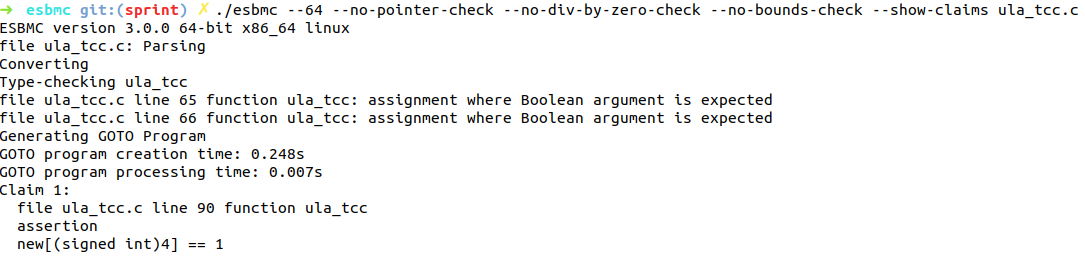
\includegraphics[scale=0.55 ]{Figuras/lista_claim.png}
%	\end{center}
%    \legend{Fonte:Própria}
%\end{figure}

%\par
%Após a listagem das claims com assertivas ser gerada, outra função, indicada na \autoref{fig:analise_claims}, é chamada para verificação de cada claim individualmente. Para cada claim, ocorre a chamada do ESBMC, utilizando as opções \texttt{$--$no-pointer-check}, \texttt{$--$no-div-by-zero-check} e \texttt{$--$no-bounds-check}, juntamente com a opção \texttt{$--$unwind} em que realiza o número de desdobramentos dos laços no código analisado. 

%\par
%Contudo, dependendo da complexidade da assertiva, faz-se necessário aumentar o número de desdobramentos que, por padrão são dez, conforme análise experimentais. A função é chamada na Linha $11$ da \autoref{fig:analise_claims} e após a análise da claim é realizado a busca do resultado e exibição caso seja uma propriedade violada.

%\par
%Desta forma o ESBMC realiza apenas a checagem necessária dentro da assertiva, evitando que outros parâmetros sejam verificados, sem a devida necessidade do mesmo. Ao final de todos os desdobramentos é apresentado o resultado, apresentado na \autoref{fig:resultado}, sendo positiva (sem erros) ou negativa (com violação de propriedades), dependendo da assertiva e do código analisado. Este processo se repete até a lista de assertivas ser finalizada.

%\begin{figure}[H]
%\caption{\label{fig:analise_claims}Pseudocódigo da função de análise das claims.}
%	\begin{center}
%    \begin{minipage}{0.7\textwidth}
%    \begin{lstlisting}       
%VAR
%contador1: inteiro
%contador2: inteiro
%resultado: lista
%
%FUNCAO esbmc_claims: lista, arquivo
%  contador1<-0
%  contador2<-0
%  busca pelo nome da funcao no arquivo
%  ENQUANTO contador < lista FACA
%    saida<-Executa comando de analise da claim numerada na %lista
%    ENQUANTO contador2 < saida
%      Regex busca se a propriedade foi violada
%      SE propriedade foi violada ENTAO
%         Pula para linha da violação
%	       Adiciona o erro ao resultado       
%      FIM-SE  
%    FIM-ENQUANTO
%  FIM-ENQUANTO
%FIM-FUNCAO
%    \end{lstlisting}
%    \end{minipage}
%	\end{center}
%    \legend{Fonte: Própria.}
%\end{figure}

%\begin{figure}[H]
%	\begin{center}
%    \caption{\label{fig:resultado}Imagem de apresentação do resultado da ferramenta.}
%	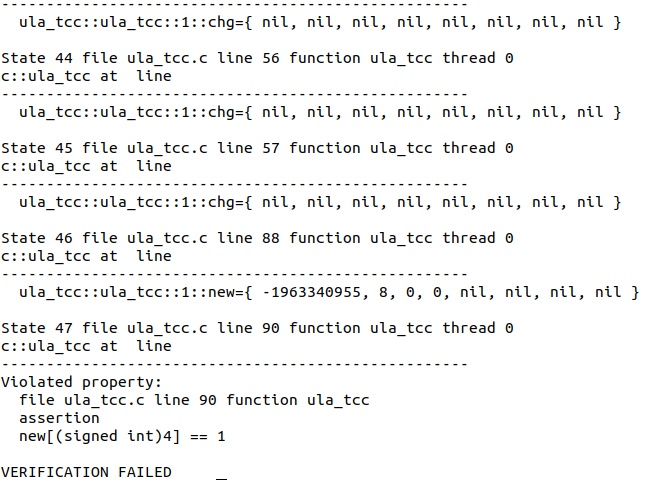
\includegraphics[scale=0.6]{Figuras/erro_assert.png}
%	\end{center}
%    \legend{Fonte:Própria}
%\end{figure}

%++++++++++++++++++++++++++++++++++++++++++++++++++++++++++
%==========================================================
%Método multiplas transformações
%==========================================================
%++++++++++++++++++++++++++++++++++++++++++++++++++++++++++
\subsection{Método multiplas transformações}
%==========================================================
%Visão geral do método multiplas transformações
%==========================================================
%\subsection{Visão geral do método multiplas transformações}
%\par
%O método proposto consiste na tradução de um código em VHDL para linguagem C e posteriormente a análise de deste programa, com base nas assertivas inseridas em um arquivo externo.  Inicialmente o código em VHDL é passado para ferramenta juntamente com outro arquivo contendo as variáveis de entrada, saída, pré-condições e pós-condições. Seguidamente é passado para duas ferramenta de tradução, inicialmente para Verilog que é instrumentado durante a execução e posteriormente traduzido para C. Após as traduções, as pré-condições e pós-condições, conforme o arquivo, são adicionadas ao códigos C e o mesmo é analisado pela ferramenta ESBMC. Caso alguma condição seja violada, o contra exemplo é apresentado ao usuário.

%========================
%Código VHDL e arquivo externo
%========================
\subsubsection{Código VHDL e arquivo externo}
\label{cap:vhdl_assertivas}

A primeira etapa do método consiste inicialmente no código VHDL a ser analisado, juntamente com o arquivo contendo as informações de entradas e saídas do código e também as pré-condições, que são condições que devem ser verdadeira antes da execução de um algum código ou trecho de código, e pós-condições que são condições declaradas e devem ser verdadeiras após a execução de um código ou trecho de código.

\par
O arquivo, \autoref{fig:arquivo_externo}, deve conter todas as variáveis de entrada e saída do código VHDL, apenas o nome da variável em ambos os casos. As variáveis de entrada são declaradas na linha \textbf{INPUT} e as variáveis de saída são declaradas na linha \textbf{OUTPUT}. Nas linhas seguintes são informadas as pré-condições e pós-condições que serão introduzidas ao código em etapas posteriores dos processos.

\begin{figure}[H]
\caption{\label{fig:arquivo_externo} Exemplo de arquivo externo.}
	\begin{center}
    \begin{minipage}{0.8\textwidth}
    \begin{lstlisting}       
INPUT:A==0,B==1,Binvertido==1,Op1==0
OUTPUT:Resultado
PRECONDITION:
POSTCONDITION:Resultado== 0
    \end{lstlisting}
    \end{minipage}
	\end{center}
    \legend{Fonte: Própria.}
\end{figure}

\par
Em comparação ao método anterior, as diferenças consistem principalmente em as assertivas não estarem mais presentes diretamente no código VHDL, desta forma, o mesmo é utilizado apenas nas etapas de tradução. A principal vantagem é a não necessidade de elementos comentados ao código VHDL e com isso o código fica mais legível e também sem a necessidade de modificação ou inserção de trecho para funcionamento da ferramenta em questão.

%===================================
%Tradução de VHDL para C e instrumentações de código
%===================================
\subsubsection{\label{cap:traducao}Tradução de VHDL para C e instrumentações de código}

\par
A primeira etapa é a tradução de código entre VHDL para C, contudo, diferente do demonstrado no primeiro método, onde apenas uma única ferramenta realizava a tradução, nesta nova reformulação do método faz a utilização de duas ferramentas de tradução, inicialmente para Verilog e uma segunda ferramenta faz a tradução para C. Isso possibilita uma um aumento no potencial da tradução, contudo, devido ao uso de duas ferramentas, alguns erros ainda podem ser verificados na tradução.

\par
Devido ao uso das ferramentas, também é necessário mais uma etapa de instrumentação, sendo uma após a tradução para Verilog e outra após a tradução para C. A primeira instrumentação modifica o código para que segunda ferramenta de tradução possa executar a tradução corretamente e a segunda instrumentação adiciona as assertivas, de acordo com o introduzido no arquivo citado na seção anterior. Nas próximas subseções serão explicados com mais detalhes as traduções e as instrumentações.

%================================================
%Tradução para Verilog e instrumentação de código
%================================================
\subsubsubsection{Tradução para Verilog e instrumentação de código}

\par
A primeira ferramenta de tradução utilizada, chamada VHD2Vl\cite{vhd2vl}, realiza a tradução do código VHDL para o código Verilog. O principal motivo de utilizar esta ferramenta deve-se a apresentar melhores resultados na tradução dos códigos, contudo, também apresenta algumas questões a serem observadas nas traduções. 

\par
Entre estas observações esta encontra-se a utilização das estruturas de std\_logic, std\_logic\_vector, integer e boolean. Também permite a utilização clock events das estruturas de controle, como if, elsif, else, case. A ferramenta também permite a instância de módulos no código VHDL, contudo o mesmo é ignorado na tradução o que causa erros de análise. Também é ignorado qualquer assertiva existente no código, tornando assim, mais necessário um arquivo externo com assertivas e condições a serem adicionadas ao texto\cite{vhd2vl}. 


\begin{figure}[H]
\caption{\label{fig:codigo_verilog} Código da \autoref{fig:code_exemplo} traduzido pela ferramenta Vhd2vl.}
	\begin{center}
    \begin{minipage}{0.7\textwidth}
    \begin{lstlisting}
[...]
module Ula_tcc(
input wire A,
input wire B,
input wire Binvertido,
input wire Op1,
output reg Resultado
);
reg and_port;
reg or_port;
reg mux2x1;
  always @(A, B, Binvertido, Op1) begin
    if((Binvertido == 1'b0)) begin
      mux2x1 <= B;
    end
    else begin
      mux2x1 <=  ~B;
    end
    and_port <= A & mux2x1;
    or_port <= A | mux2x1;
    if((Op1 == 1'b0)) begin
      Resultado <= and_port;
    end
    else if((Op1 == 1'b1)) begin
      Resultado <= or_port;
    end
  end
endmodule
    \end{lstlisting}
    \end{minipage}
	\end{center}
    \legend{Fonte: Própria.}
\end{figure}

\par
Contudo, o código conforme apresentado acima, não pode ser traduzido para C, pois está fora do padrão aceito pela ferramenta V2c, que realiza a tradução de verilog para C. Com isso é necessária uma instrumentação de código para que o mesmo possa ser traduzido. Esta instrumentação consiste na alteração dos modo de declaração das variáveis, na alteração de palavras chaves utilizadas no verilog e na busca de elementos que estejam dentro com escopo \textit{always@()}, que contém a arquitetura do código.

\begin{figure}[H]
\caption{\label{fig:codigo_verilog_declaracao} Diferença da declaração das variáveis após a intrumentação.}
	\begin{center}
    \begin{minipage}{0.7\textwidth}
    \begin{lstlisting}
[...]
module Ula_tcc(
input wire A,
input wire B,
input wire Binvertido,
input wire Op1,
output reg Resultado
);
[...]
    \end{lstlisting}
    \end{minipage}
    \legend{(a)}
    \begin{minipage}{0.7\textwidth}
    \begin{lstlisting}
module Ula_tcc(A,B,Binvertido,Op1,Resultado);
input wire A;
input wire B;
input wire Binvertido;
input wire Op1;
output Resultado;
reg Resultado;
[...]
    \end{lstlisting}
    \end{minipage}
    \legend{(b)}
	\end{center}
    \legend{Fonte: Própria.}
\end{figure}

\par
A primeira adaptação a ser feita é na declaração das variáveis. Conforme a \autoref{fig:codigo_verilog_declaracao}(a) apresenta a declaração após a tradução e a \autoref{fig:codigo_verilog_declaracao}(b) apresenta após a instrumentação. As mudanças consistem em o nome das variáveis serem declaradas como uma espécie de parâmetro e logo abaixo seus respectivos tipos, fora do modulo. Outra alteração é com relação ao \textbf{Output reg}, onde primeiro se declara como saída e depois como reg a mesma variável, como apresentado na linha 7 e 8 da \autoref{fig:codigo_verilog_declaracao}(b) em relação a linha 7 da \autoref{fig:codigo_verilog_declaracao}(a). 

\par
Outra alteração necessário é que nenhuma variável seja declarada dentro do modulo Always@(), pois gera a não tradução do código por parte da ferramenta. Com isso toda e qualquer variável que venha a ser utilizado durante a execução do código deve ser declarado antes do modulo always@(), conforme \autoref{fig:codigo_verilog_always}. E outra alteração consiste nas palavras reservadas, visto que verilog utiliza a palavra \textbf{define} para definição de constante. Esta alteração é importante, pois evita que o código seja traduzido de maneira errada. 

\begin{figure}[H]
\caption{\label{fig:codigo_verilog_always} Declaração de variáveis anteriores ao modulo Always@()}
	\begin{center}
    \begin{minipage}{0.7\textwidth}
    \begin{lstlisting}
[...]
reg and_port;
reg or_port;
reg mux2x1;

always @(A, B, Binvertido, Op1) begin
    [...]
endmodule
    \end{lstlisting}
    \end{minipage}
	\end{center}
    \legend{Fonte: Própria.}
\end{figure}

\par

%================================================
%Tradução para Verilog e instrumentação de código
%================================================
\subsubsubsection{Tradução para C e adição das pre-condições e pós-condições.}

\par
A segunda parte da tradução é realizada pela ferramenta V2C \cite{mukherjee2016v2c}. Como citado anteriormente, após a instrumentação no código verilog o mesmo pode ser traduzido para C, conforme apresentado na \autoref{fig:codigo_C}. Após a tradução o código recebe as assertivas e inicializações de variáveis.  

\par
Toda parte de arquitetura do código VHDL após a tradução para C é colocada em uma função de mesmo nome do arquivo. Também é definido uma \textit{struct} que contém as variáveis que foram declaradas como \textit{output} e também variáveis que tenham sido declaradas para serem utilizadas na execução da arquitetura, como os sinais por exemplo. As variáveis de entrada são declaradas na função main() e são repassadas como parâmetros da função. 

\par
A necessidade desta \textit{struct} deve-se ao fato de que estas variáveis podem ter seus valores alterados em tempo de execução. Devido a este fato, variáveis são criadas para armazenar valores antigos e também receber novos valores, como ocorre nas linhas treze, catorze, quinze e dezeseis da \autoref{fig:codigo_C}. Nota-se que estas variáveis possuem o mesmo nome das variáveis da \textit{struct}, com a adição do sufixo \_old. 

\par
Após a etapa de conversão para linguagem C ocorre uma nova etapa de instrumentação de código, onde as assertivas serão introduzidas ao código C. Para isso faz-se necessário a utilização do arquivo de pré-condições e pós-condições passado para ferramenta juntamente com o código VHDL e apresentado na \autoref{fig:arquivo_externo}.  

\begin{figure}[H]
\caption{\label{fig:codigo_C} Código C traduzido após a intrumentação no verilog.}
	\begin{center}
    \begin{minipage}{0.7\textwidth}
    \begin{lstlisting}
#include <stdio.h>
#include <assert.h>
#define TRUE 1
#define FALSE 0
struct state_elements_Ula_tcc{
_Bool Resultado;
_Bool and_port;
_Bool or_port;
_Bool mux2x1;
};
void Ula_tcc(_Bool A, _Bool B, _Bool Binvertido, _Bool Op1, _Bool *Resultado){
  struct state_elements_Ula_tcc  sUla_tcc;
  _Bool Resultado_old;
  _Bool and_port_old;
  _Bool or_port_old;
  _Bool mux2x1_old;
  mux2x1_old = sUla_tcc.mux2x1;
  and_port_old = sUla_tcc.and_port;
  or_port_old = sUla_tcc.or_port;
  Resultado_old = sUla_tcc.Resultado;
  if((unsigned char)Binvertido == 0){
    sUla_tcc.mux2x1 = B;
  }
  else{
    sUla_tcc.mux2x1 = !B;
  }
  sUla_tcc.and_port = A && mux2x1_old;
  sUla_tcc.or_port = A || mux2x1_old;
  if((unsigned char)Op1 == 0){
    sUla_tcc.Resultado = and_port_old;
  }
  else{
    if((unsigned char)Op1 == 1){
      sUla_tcc.Resultado = or_port_old;
    }
  }
}
void main() {
_Bool A;
_Bool B;
_Bool Binvertido;
_Bool Op1;
_Bool Resultado;
Ula_tcc(A, B, Binvertido, Op1, &Resultado);
}
    \end{lstlisting}
    \end{minipage}
	\end{center}
    \legend{Fonte: Própria.}
\end{figure}

\par
Para a instrumentação é necessário a utilização de funções próprias do analisador, neste caso o ESBMC \cite{esbmc} e estas funções são: \textbf{ESBMC\_assume()}, \textbf{\_\_VERIFIER\_nondet\_int()} e \textbf{\_\_VERIFIER\_nondet\_bool()}. A função \textbf{ESBMC\_assume()} permite que uma variável assuma um valor especifico. As funções \textbf{\_\_VERIFIER\_nondet\_int()} e \textbf{\_\_VERIFIER\_nondet\_bool()} modelam valores inteiros e booleanos não deterministicos respectivamente.

\par
A função ESBMC\_assume() é utilizada quando alguma variável foi inicializada no arquivo, desta forma a mesma é inicializada no código. Na linha 1 da \autoref{fig:arquivo_externo} é declarada variável inicializada e das linhas 21 a 24 da \autoref{fig:codigo_C_assert} é utilizado as funções para declaração das variáveis. Desta forma,  estes valores são definidos para aquela variável no tempo de execução da análise. 

\par
A importância das funções \textbf{\_\_VERIFIER\_nondet\_int()} e \textbf{\_\_VERIFIER\_nondet\_bool()} no desenvolvimento do método é evitar que um determinado estado do código não possa ser alcançado, devido a não inicialização de variáveis. Estas funções são utilizadas nas variáveis de entrada não inicializadas e as outras variáveis que não são inputs e nem outputs. Na \autoref{fig:codigo_C_assert}, linhas 48 a 51 apresenta o uso desta função.

\par
Em outras palavras, na instrumentação de código é realizado a adição das assertivas do modelo utilizado no arquivo para o modelo utilizado em linguagem C, além como de outras funções que possam ser utilizados pelo VHDL. Ao final da instrumentação o código C fica disponível para que possa ser dado como entrada para outras ferramentas de verificação de código e não apenas o ESBMC. 

\begin{figure}[H]
\caption{\label{fig:codigo_C_assert} Código C adição das assertivas.}
	\begin{center}
    \begin{minipage}{0.7\textwidth}
    \begin{lstlisting}
#include <stdio.h>
#include <assert.h>
#define TRUE 1
#define FALSE 0
struct state_elements_Ula_tcc{
_Bool Resultado;
_Bool and_port;
_Bool or_port;
_Bool mux2x1;
};
void Ula_tcc(_Bool A, _Bool B, _Bool Binvertido, _Bool Op1, _Bool *Resultado){
  struct state_elements_Ula_tcc  sUla_tcc;
  _Bool Resultado_old;
  _Bool and_port_old;
  _Bool or_port_old;
  _Bool mux2x1_old;
  mux2x1_old = sUla_tcc.mux2x1;
  and_port_old = sUla_tcc.and_port;
  or_port_old = sUla_tcc.or_port;
  Resultado_old = sUla_tcc.Resultado;
  __ESBMC_assume(A==0);
  __ESBMC_assume(B==1);
  __ESBMC_assume(Binvertido==1);
  __ESBMC_assume(Op1==0);
  if((unsigned char)Binvertido == 0){
    sUla_tcc.mux2x1 = B;
  }
  else{
    sUla_tcc.mux2x1 = !B;
  }
  sUla_tcc.and_port = A && mux2x1_old;
  sUla_tcc.or_port = A || mux2x1_old;
  if((unsigned char)Op1 == 0){
    sUla_tcc.Resultado = and_port_old;
  }
  else
    if((unsigned char)Op1 == 1){
      sUla_tcc.Resultado = or_port_old;
    }
    __ESBMC_assert(sUla_tcc.Resultado == 0,"Teste");
}
void main() {
_Bool A;
_Bool B;
_Bool Binvertido;
_Bool Op1;
_Bool Resultado;
A=__VERIFIER_NONDET_BOOL();
B=__VERIFIER_NONDET_BOOL();
Binvertido=__VERIFIER_NONDET_BOOL();
Op1=__VERIFIER_NONDET_BOOL();
Ula_tcc(A, B, Binvertido, Op1, &Resultado);
}
    \end{lstlisting}
    \end{minipage}
	\end{center}
    \legend{Fonte: Própria.}
\end{figure}
%=============================================
%Verificação de assertvas usando model checker
%=============================================
\subsection{\label{sec:verificacao}Verificação de assertivas usando \textit{Model Checker}}

\par
O \textit{model checker} adotado no desenvolvimento de método é o ESBMC~\cite{cordeiro2012smt} na versão $6.0.0$ e conforme explicado na Seção~\ref{cap:bounded}, esta ferramenta recebe como entrada um código C ou C$++$ e também utiliza solucionadores SMT para análise do programa. 

\par
Para verificação pode ser utilizado o métodos de análise, chamado indução-k. A indução-k é o meio principal de verificação, juntamente com o mesmo é adicionado as seguintes opções, estas que o analisador trabalhe diretamente e unicamente com as assertivas, evitando que outros fatores possam ser analisados no código: 
\begin{itemize} 
    \item \textbf{$--$no-pointer-check:} para não realizar a checagem de ponteiros no código; 
    \item \textbf{$--$no-div-by-zero-check:} para não realizar a checagem de divisões por zero no código; e 
    \item \textbf{$--$no-bounds-check:} para não realizar a checagem de array bounds no código. 
\end{itemize} 

\par
\textcolor{red}{Desta forma o ESBMC realiza apenas a checagem necessária dentro da assertiva, evitando que outros parâmetros sejam verificados, sem a devida necessidade do mesmo. O ESBMC utilizando a técnica de indução-k realiza a análise das assertivas em cada código, considerando as pré condições e também os valores determinados para as variáveis dentro o código através do ESBMC\_assume(). Ao final de todos os desdobramentos é apresentado o resultado, sendo positiva (sem erros) ou negativa (com violação de propriedades), dependendo da assertiva e do código analisado.}

\section{Resumo do capitulo}
\textcolor{red}{Neste capitulo foi apresentado os dois métodos de tradução composto pelo método de múltiplas traduções, na qual é utilizado duas ferramentas de tradução, e pelo método de tradução direta que utiliza apenas uma ferramenta e faz a conversão direta de VHDL para linguagem C. Também foi mostrado a ferramenta de análise chamada ESBMC e de que forma ela é utilizada para verificação dos códigos.} 